\documentclass{ximera}

\newcommand{\RR}{\mathbb R}
\renewcommand{\d}{\,d}
\newcommand{\dd}[2][]{\frac{d #1}{d #2}}
\renewcommand{\l}{\ell}
\newcommand{\ddx}{\frac{d}{dx}}
\newcommand{\dfn}{\textbf}
\newcommand{\eval}[1]{\bigg[ #1 \bigg]}



\outcome{Review differentiation.}
\outcome{Review integration.}
\outcome{Use algebra to manipulate the integrand.}
\outcome{Determine when a function is a composition of two or more functions.}
\outcome{Calculate indefinite and definite integrals requiring complicated substitutions.}
\outcome{Recognize common patterns in substitutions.}
\outcome{Evaluate indefinite and definite integrals through a change of variables.}

\title[Dig-In:]{A review of integration}

\begin{document}
\begin{abstract}
  We review differentiation and integration.
\end{abstract}
\maketitle


\section{Basic derivatives and antiderivatives}

Let's get started. Recall the derivative rules:

\begin{theorem}[Basic Derivative Rules]\index{derivative rules}
  Let $n\ne 0$, $k$ be a constant and $a>0$.
\begin{itemize}
\item $\ddx k =0$
\item $\ddx x^n  = n x^{n-1}$
\item $\ddx e^x = e^x$
\item $\ddx a^x = a^x\ln(a)$
\item $\ddx \ln(x) = \frac{1}{x}$
\item $\ddx \sin(x) = \cos(x)$
\item $\ddx \cos(x) = -\sin(x)$  
\item $\ddx \tan(x) = \sec^2(x)$  
\item $\ddx \sec(x) = \sec(x)\tan(x)$ 
\item $\ddx \csc(x) = -\csc(x)\cot(x)$
\item $\ddx \cot(x) = -\csc^2(x)$
\item $\ddx \arcsin(x) = \frac{1}{\sqrt{1-x^2}}$
\item $\ddx \arccos(x) = \frac{-1}{\sqrt{1-x^2}}$
\item $\ddx \arctan(x) =\frac{1}{1+x^2}$
\item $\ddx \arcsec(x) = \frac{1}{|x|\sqrt{x^2-1}}$ for $|x|>1$
\item $\ddx \arccsc(x) = \frac{-1}{|x|\sqrt{x^2-1}}$ for $|x|>1$
\item $\ddx \arccot(x) = \frac{-1}{1+x^2}$
\item $\ddx \left( f(x) + g(x) \right) = f'(x) + g'(x)$
\item $\ddx \left( f(x) \cdot g(x) \right) = f(x)g'(x) + f'(x)g(x)$
\item $\ddx\frac{f(x)}{g(x)} = \frac{f'(x)g(x) - f(x)g'(x)}{g(x)^2}$
\item $\ddx f(g(x)) = f'(g(x)) \cdot g'(x)$
\end{itemize}
%\end{multicols}
\end{theorem}

\begin{question} 
  What is the derivative of $\arcsin\left(\frac{x}{a}\right)$ with respect to $x$?
  \begin{prompt} 
    \[
    \ddx \arcsin\left(\frac{x}{a}\right) = \answer{1/(a \sqrt{1-(x/a)^2})}
    \]
  \end{prompt}
\end{question}

When computing definite integrals, the Fundamental Theorem of Calculus
says:

\begin{theorem}[Fundamental Theorem of Calculus]\index{Fundamental Theorem of Calculus}
  Let $f$ be continuous on $[a,b]$. If $F$ is \textbf{any}
  antiderivative of $f$, then
  \[
  \int_a^b f(x)\d x = F(b)-F(a).
  \]
\end{theorem}

The Fundamental Theorem of Calculus allows us to compute
integrals by ``undoing'' the derivative.

\begin{theorem}[Basic Indefinite Integrals]\index{antiderivatives}\index{indefinite integral}\hfil
\begin{itemize}
\item $\int k \d x= \answer[given]{k x}+C$
\item $\int x^n \d x= \answer[given]{\frac{x^{n+1}}{n+1}}+C\qquad(n\ne-1)$
\item $\int e^x \d x= \answer[given]{e^x} + C$
\item $\int a^x \d x= \answer[given]{\frac{a^x}{\ln(a)}}+C$
\item $\int \frac{1}{x} \d x= \ln|x|+C$
\item $\int \cos(x) \d x = \answer[given]{\sin(x)} + C$
\item $\int \sin(x) \d x = \answer[given]{-\cos(x)} + C$  
\item $\int \tan(x) \d x = -\ln|\cos(x)| + C$
\item $\int \sec^2(x) \d x = \answer[given]{\tan(x)} + C$
\item $\int \csc^2(x) \d x = \answer[given]{-\cot(x)} + C$
\item $\int \sec(x)\tan(x) \d x = \answer[given]{\sec(x)} + C$
\item $\int \csc(x)\cot(x) \d x = \answer[given]{-\csc(x)} + C$
\item $\int \frac{1}{x^2+1}\d x = \answer[given]{\arctan(x)} + C$
\item $\int \frac{1}{\sqrt{1-x^2}}\d x= \answer[given]{\arcsin(x)}+C$
\end{itemize}
\end{theorem}

Whenever you compute an indefinite integral, you can always check your
work by taking the derivative. In particular, this means that if you
are given choices for the antiderivative, you can check simply by
taking the derivative. Note, there are always many choices for
antiderivative, as they may differ by a constant.

\begin{question}
  Which of the following are an antiderivative of $\frac{1}{x\ln(x^2)}$?
  \begin{selectAll}
    \choice[correct]{$\frac{1}{2}\ln(\ln(x^2))$}
    \choice[correct]{$\frac{\ln(2) + \ln(\ln(x))}{2}$}
    \choice[correct]{$\frac{\ln(\ln(x))}{2}$}
    \choice[correct]{$\frac{\ln(7\cdot \ln(x))}{2}$}
    \choice[correct]{$\frac{\ln(\ln(x^3))}{2}$}
  \end{selectAll}
\end{question}

\section{The substitution formula}

While antiderivatives are often tricky to compute, the substitution
formula is a tool that can help:

\begin{theorem}[Integral Substitution Formula] 
If $g$ is differentiable on the interval $[a,b]$ and $f$ is
differentiable on the interval $[g(a),g(b)]$, then
\[
\int_a^b f'(g(x)) g'(x) \d x =\int_{g(a)}^{g(b)} f'(g) \d g.
\]
\end{theorem}

The substitution formula allows us to change the form of a novel
integral, so that we can evaluate it using forms we know.

\begin{example}
  Letting $a>0$, compute:
  \[
  \int \frac{1}{\sqrt{a-x^2}} \d x
  \]
  \begin{explanation}
    Looking over our basic integral formulas, we see that this is similar to
    \[
    \int \frac{1}{\sqrt{1-x^2}}\d x= \answer[given]{\arcsin(x)}+C.
    \]
    So our goal will be to somehow ``transform'' the integral we are
    trying to compute to one that is similar to the one we know how to
    compute. First note
    \[
    \int \frac{1}{\sqrt{a-x^2}} \d x  =
    \int \frac{1}{\sqrt{\answer[given]{a}\left(1-\frac{x^2}{a}\right)}} \d x
    \]
    and since $a>0$, we may write:
    \[
    \int \frac{1}{\sqrt{a\left(1-\frac{x^2}{a}\right)}} \d x=
    \int \frac{1}{\answer[given]{\sqrt{a}}\cdot \sqrt{1-\left(\frac{x}{\sqrt{a}}\right)^2}} \d x
    \]
    Recalling that we may always pull constants out of integrals, write:
    \[
    \int \frac{1}{\sqrt{a}\cdot \sqrt{1-\left(\frac{x}{\sqrt{a}}\right)^2}} \d x = 
    \answer[given]{\frac{1}{\sqrt{a}}}\int \frac{1}{\sqrt{1-\left(\frac{x}{\sqrt{a}}\right)^2}} \d x 
    \]
    Ah! Now our integral looks more like one we can do. We will now
    proceed using substitution. Set $g = \frac{x}{\sqrt{a}}$, and write with me
    \begin{align*}
      \d g &= \frac{\d x}{\sqrt{a}},\\
      \d x &= \sqrt{a}\d g,
    \end{align*}
    and now
    \begin{align*}
    \frac{1}{\sqrt{a}}\int \frac{1}{\sqrt{1-\left(\frac{x}{\sqrt{a}}\right)^2}} \d x &=
    \frac{1}{\sqrt{a}}\int \frac{1}{\sqrt{1-g^2}} \sqrt{a} \d g\\
    &=\int \frac{1}{\sqrt{1-g^2}}\d g\\
    &=\arcsin(g) + C\\
    &=\arcsin\left(\frac{x}{\sqrt{a}}\right) + C.
    \end{align*}
  \end{explanation}
\end{example}





\begin{question}
  Letting $a$ be nonzero, what is the antiderivative of $\frac{1}{a +
    x^2}$?
  \begin{prompt}%%BADBAD BADBAD BADBAD
    \[
    \int \frac{1}{a + x^2} \d x = \answer{(1/\sqrt{a}) \arctan(x/\sqrt{a})}+C
    \]
  \end{prompt}
  \begin{hint}
    Try to use the same procedure used in the example above.
  \end{hint}
\end{question}


Let's see another example involving substitution:


\begin{example}
Compute:
\[
\int_0^{16} \sqrt{4 - \sqrt{x}} \d x
\]
\begin{explanation}
While it is not obvious at all, let us try the substitution
\[
g = \sqrt{x}.
\]
Then
\begin{align*}
\d g &= \answer[given]{\frac{1}{2 \sqrt{x}}} \d x,\\
\d x &= 2 \sqrt{x} \d g = 2g \d g,
\end{align*}
and so
\begin{align*}
\int_0^{16} \sqrt{4 - \sqrt{x}} \d x &= \int_{g(0)}^{g(16)} \answer[given]{\sqrt{4-g} \cdot 2g} \d g  \\
&= \int_{\answer[given]{0}}^{\answer[given]{4}} \answer[given]{2g \sqrt{4-g}} \d g.
\end{align*}
From here we now make the second (and more obvious) substitution
\[
h = 4-g.
\]
Then $g = 4-h$, and
\begin{align*}
\d h &= - \d g,\\
\d g &= - \d h.
\end{align*}
So
\begin{align*}
\int_0^{16} \sqrt{4 - \sqrt{x}} \d x &= \int_0^4 2g \sqrt{4-g} \d g  \\
&= \int_{h(0)}^{h(4)} 2 (4-h) \sqrt{h} (-1) \d h  \\
&= - \int_{\answer[given]{4}}^{\answer[given]{0}} ( 8h^{\frac{1}{2}} - 2h^{\frac{3}{2}} ) \d h  \\
&= \int_{\answer[given]{0}}^{\answer[given]{4}} ( 8h^{\frac{1}{2}} - 2h^{\frac{3}{2}} ) \d h  \\
&= \eval{ \answer[given]{8 \left( \frac{2}{3} \right) h^{\frac{3}{2}} - 2 \left( \frac{2}{5} \right) h^{\frac{5}{2}}} }_{0}^{4}  \\
&= \left( \frac{16}{3} (4)^{\frac{3}{2}} - \frac{4}{5} (4)^{\frac{5}{2}} \right) - \left( 0 - 0 \right)  \\
&= \frac{128}{3} - \frac{128}{5}   \\
&= \frac{256}{15}.
\end{align*}
\end{explanation}
\end{example}


\section{Algebra to the rescue}

With substitution, and a little algebraic manipulation, one can
compute more integrals. In what follows, we will work many examples.
In each case below we will present a ``novel'' integral, and then use
algebra and substitution to change the form of the integral to one
we know.

Sometimes it is best to ``expand'' the integrand.

\begin{example}
  Compute:
  \[
  \int (7-x^2)^2 \d x
  \]
  \begin{explanation}
    Let's start by expanding the integrand:
    \[
    \int (7-x^2)^2 \d x  = \int \answer[given]{49 - 14x^2 + x^4} \d x
    \]
    Ah, this is now easy, write with me:
    \[
    \int 49 - 14x^2 + x^4 \d x = \answer[given]{49x - \frac{14 x^3}{3} + \frac{x^5}{5}} + C
    \]
  \end{explanation}
\end{example}

Functions consisting of products of the sine and cosine can be
integrated by using substitution and trigonometric identities. These
can sometimes be tedious, but the technique is straightforward. The
basic idea in each case is to somehow take advantage of a
trigonometric identity, usually the Pythagorean identity, or a
power-reduction formula:
\begin{description}\index{Pythagorean identity}\index{power-reduction!formula}
\item[Pythagorean Identity] $\cos^2(x) + \sin^2(x) = 1$
\item[Cosine Power-Reduction] $\cos^2(x)= \frac{1+\cos(2x)}{2}$\index{cosine power-reduction}
\item[Sine Power-Reduction] $\sin^2(x) = \frac{1-\cos(2x)}{2}$\index{sine power-reduction}
\end{description}

We'll work some examples to demonstrate how to use these formulas.

\begin{example}
  Compute:
  \[
  \int (\cos(x)+\sin(x))^2\d x
  \]
  \begin{explanation}
    Let's start by expanding the integrand:
    \begin{align*}
      \int &(\cos(x)+\sin(x))^2 \d x\\
      &= \int \answer[given]{\cos^2(x) + 2\cos(x)\sin(x) + \sin^2(x)} \d x
    \end{align*}
    Now if we rearrange we can use the Pythagorean identity, write with me:
    \begin{align*}
      \int &\cos^2(x) + 2\cos(x)\sin(x) + \sin^2(x) \d x \\
      &= \int \cos^2(x) + \sin^2(x) + 2\cos(x)\sin(x) \d x\\
      &= \int \answer[given]{1 + 2\cos(x)\sin(x)} \d x
    \end{align*}
    Now we may set $g = \sin(x)$ and so
    \begin{align*}
      \d g &= \answer[given]{\cos(x)} \d x,\\
      \d x & = \frac{\d g}{\cos(x)},
    \end{align*}
    and we find
    \begin{align*}
      \int 1 + 2\cos(x)\sin(x) \d x &= \int 1 \d x + \int 2g \d g\\
      &= x + g^2 + C\\
      &= x + \answer[given]{\sin^2(x)}+C.
    \end{align*}
  \end{explanation}
\end{example}

Let's see one more example with trigonometric functions:

\begin{example}
  Compute:
  \[
  \int \frac{\sin(x) + \cos^2(x)}{\csc(x)} \d x
  \]
  \begin{explanation}
    To start, let's express everything in terms of sine and cosine:
    \begin{align*}
      \int \frac{\sin(x) + \cos^2(x)}{\csc(x)} \d x &= \int \frac{\sin(x) + \cos^2(x)}{\frac{1}{\sin(x)}} \d x\\
      &= \int \sin^2(x) + \sin(x)\cos^2(x) \d x
    \end{align*}
    if we use our power-reduction formula above, we find
    \[
    \int \answer[given]{\frac{1-\cos(2x)}{2}}+ \sin(x)\cos^2(x) \d x
    \]
    Splitting this integral up we now have
    \begin{align*}
      \int &\answer[given]{\frac{1}{2}} \d x - \int \frac{\cos(2x)}{2}\d x + \int \sin(x)\cos^2(x) \d x  \\
      &= \answer[given]{\frac{x}{2} - \frac{\sin(2x)}{4} - \frac{\cos^3(x)}{3}}+C.
    \end{align*}
  \end{explanation}
\end{example}

In a similar vein, if you have a fraction, it can help to separate the
integrand into several fractions.

\begin{example}
  Compute:
  \[
  \int \frac{6x-8}{1+x^2}\d x
  \]
  \begin{explanation}
    Write with me:
    \begin{align*}
      \int \frac{6x-8}{1+x^2}\d x &= \int \frac{\answer[given]{6x}}{1+x^2}-\frac{8}{1+x^2}\d x\\
      &= 3\int\frac{2x}{1+x^2}\d x -8\int \frac{1}{1+x^2}\d x\\
      &= 3\ln|1+x^2|\d x -8\arctan(x)+ C.\\
    \end{align*}
  \end{explanation}
\end{example}

Your old friend (or enemy!) long-division\index{long-division} can help too.

\begin{example}
  Compute:
  \[
  \int \frac{3x^2-17x +1}{x-5} \d x
  \]
  \begin{explanation}
    Now we will use long-division. Write:
    %%\[
    %% x-5\,\begin{array}[b]{@{}r@{}r} 
    %% \answer[given]{3x-2} &\\ 
    %% \cline{1-1}
    %% \Bigg)\begin{array}[t]{@{}l@{}} 3x^2-17x+1\\ 
    %%   \answer[given]{3x^2-15x} \\ 
    %%   \divrule{0}{8}  ~~~~~\answer[given]{-2x+1} \\
    %%   ~~~~~\answer[given]{-2x+10}\\
    %%   \divrule{5}{8}
    %%   ~~~~~~~~~~\answer[given]{-9}
    %% \end{array}
    %% \end{array}
    %% \]
    \begin{center}%%BADBAD
      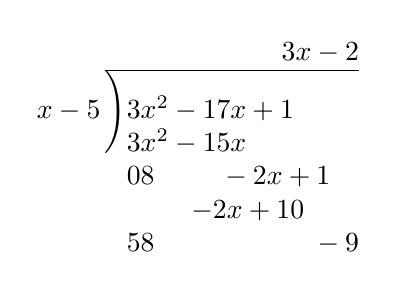
\begin{tikzpicture}[]
        \node at (0,0) {
    $x-5\,\begin{array}[b]{@{}r@{}r} 
    3x-2 &\\ 
    \cline{1-1}
    \Bigg)\begin{array}[t]{@{}l@{}} 3x^2-17x+1\\ 
      3x^2-15x \\ 
      \divrule{0}{8}  ~~~~~~~-2x+1 \\
      ~~~~~~~-2x+10\\
      \divrule{5}{8}
      ~~~~~~~~~~~~~~~~~-9
    \end{array}
    \end{array}
          $
        };
      \end{tikzpicture}
    \end{center}
    From this we see that
    \begin{align*}
      \int \frac{3x^2-17x +1}{x-5} \d x &= \int 3x-2 - \answer[given]{\frac{9}{x-5}}\d x\\
      &= \frac{3x^2}{2} - 2x -9 \ln|x-5| +C
    \end{align*}
    %Why is the rendering wrong?
  \end{explanation}
\end{example}

Finally, sometimes it helps to complete the square.\index{complete the square}

\begin{example}
  Compute:
  \[
  \int \frac{1}{x^2-17x +1}\d x
  \]
  \begin{explanation}
    To start, let's complete the square in the denominator. Write with me:
    \begin{align*}
      \int &\frac{1}{x^2-17x +1} \d x \\
      &=  \int \frac{1}{x^2-17x +\left(\frac{17}{2}\right)^2 + 1 - \left(\frac{17}{2}\right)^2} \d x\\
      &=  \int \frac{1}{\left(\answer[given]{x-\frac{17}{2}}\right)^2 + 1 - \left(\frac{17}{2}\right)^2} \d x
    \end{align*}
    At this point set $g= x-\frac{17}{2}$, so $\d g = \d x$ and we have
    \begin{align*}
    \int &\frac{1}{g^2 + 1 - \left(\frac{17}{2}\right)^2} \d g \\
    &= \frac{1}{\sqrt{1 - \left(\frac{17}{2}\right)^2}} \arctan\left(\frac{g}{\sqrt{1 - \left(\frac{17}{2}\right)^2}}\right)\\
    &= \frac{1}{\sqrt{1 - \left(\frac{17}{2}\right)^2}} \arctan\left(\frac{\answer[given]{x-\frac{17}{2}}}{\sqrt{1 - \left(\frac{17}{2}\right)^2}}\right).
    \end{align*}
  \end{explanation}
\end{example}

As a final strategy, please, when you are learning, feel free to find
the answer using a computer. This may seem like ``cheating'' but you
can gain insight from this too.
\begin{quote}
  \textbf{Always remember: Don't give up.}
\end{quote}
\end{document}
